% IGC architecture / gradient-flow figure --- DRAFT to merge into the main paper.
% Self-contained: compile with `pdflatex igc_architecture.tex`.
% The figure (Fig.~\ref{fig:igc-gradflow}) is drawn in TikZ so it stays vector/editable
% and can be lifted straight into the paper's figure environment.
%
% Author: Mus mbayramo@stanford.edu
\documentclass[11pt]{article}
\usepackage[margin=1in]{geometry}
\usepackage{amsmath,amssymb}
\usepackage{tikz}
\usetikzlibrary{arrows.meta,positioning,fit,backgrounds,calc}
\usepackage{xcolor}

\definecolor{gradc}{RGB}{22,163,74}
\definecolor{datac}{RGB}{107,114,128}
\definecolor{actc}{RGB}{217,119,6}
\definecolor{stopc}{RGB}{220,38,38}

\tikzset{
  box/.style   = {draw, rounded corners=3pt, minimum width=2.7cm, minimum height=0.95cm,
                  align=center, font=\small, inner sep=3pt},
  train/.style = {box, fill=blue!7,  draw=blue!55},
  frozen/.style= {box, fill=gray!8,  draw=gray!55},
  lossb/.style = {box, fill=teal!8,  draw=teal!60},
  unw/.style   = {box, fill=gray!5,  draw=gray!45, dashed, font=\footnotesize,
                  minimum width=5.3cm, text=gray!55!black},
  data/.style  = {-{Latex[length=2mm]}, datac, thick},
  grad/.style  = {-{Latex[length=2mm]}, gradc, very thick},
  act/.style   = {-{Latex[length=2mm]}, actc, thick, dashed},
  stop/.style  = {-{Latex[length=2mm]}, stopc, thick, dashed},
  elab/.style  = {font=\scriptsize, inner sep=1.5pt},
}

\title{\textbf{IGC: Training Architecture and Gradient Flow}\\[2pt]
       \large (draft figure --- merge into the main paper)}
\author{Mus Bayramov}
\date{}

\begin{document}
\maketitle

\section{Training decomposition}

IGC is trained as \emph{three separate supervised/RL ``islands,'' never end-to-end}. This is a
deliberate design choice (and is what the current implementation enforces with hard
stop-gradients), not an accident of the code:

\begin{itemize}\itemsep2pt
  \item \textbf{State Encoder (M1)} is the only module trained end-to-end \emph{within itself}: a
  causal-LM next-token loss backpropagates through the entire backbone under a single optimizer.
  It learns a representation of a Redfish observation (a GET/HEAD response).
  \item \textbf{State Pooler (M2)} learns a compact bottleneck by reconstructing the encoder's last
  hidden state; the backbone runs under \texttt{no\_grad}, so the reconstruction gradient reaches
  only the pooler.
  \item \textbf{Policy (M6)} is trained by temporal-difference RL (with hindsight experience replay)
  and updates \emph{only} the action-value network. The encoder is \textbf{frozen} during RL: the
  observation embedding is detached at the environment boundary, so no RL gradient ever flows back
  into the representation. This keeps the (expensive, language-pretrained) representation stable
  while the policy explores.
\end{itemize}

Reward and action edges are \emph{non-differentiable} (they carry data into the TD target, not
gradient). The evaluator (M4) and world-model (M5) are part of the planned design; the accepted
pointer-style policy head is implemented but not yet wired into the training loop. Figure
\ref{fig:igc-gradflow} makes the gradient boundaries explicit.

\begin{figure}[h]
\centering
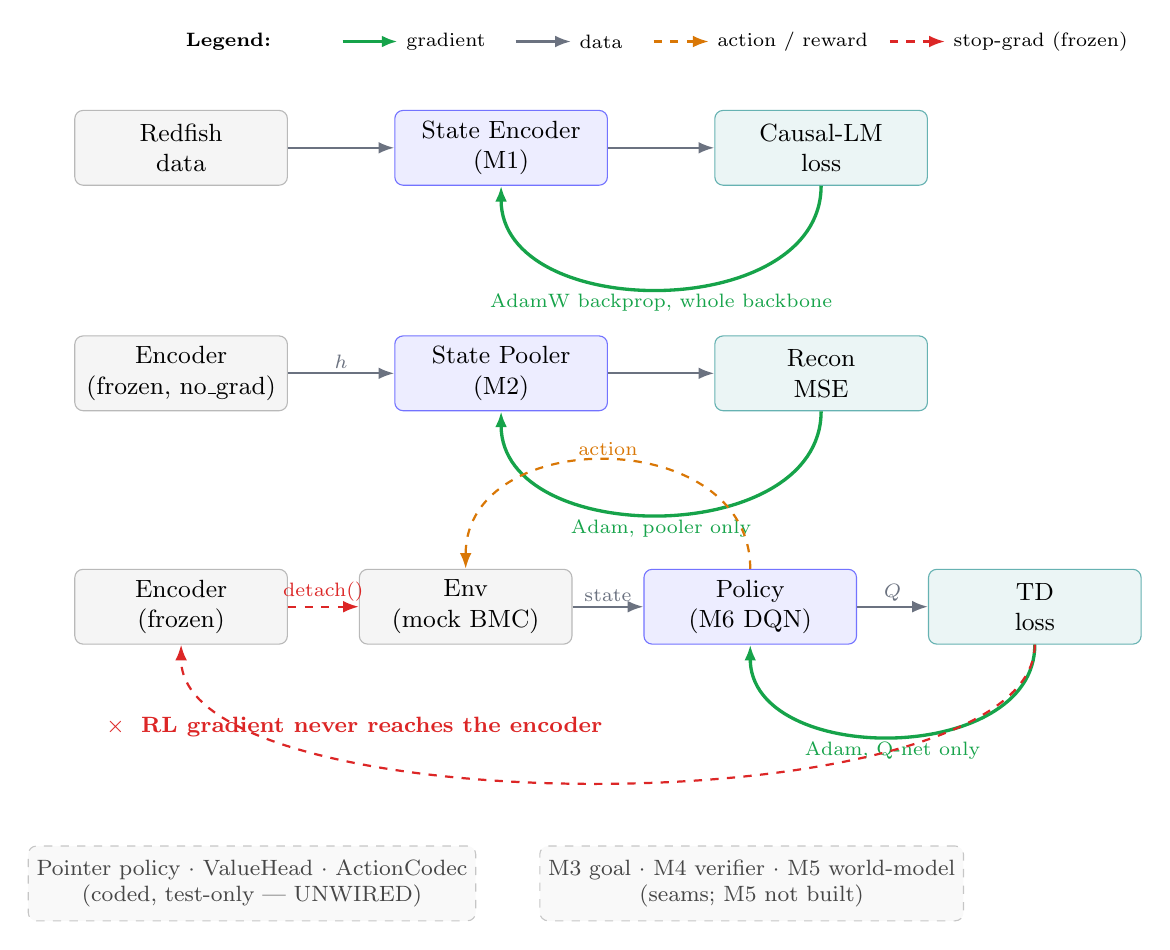
\begin{tikzpicture}[node distance=1.3cm and 1.35cm]

% ---- legend ----
\node[elab, anchor=west] (lg) at (0,1.35) {\textbf{Legend:}};
\draw[grad] (2.05,1.35) -- (2.75,1.35); \node[elab,anchor=west] at (2.8,1.35) {gradient};
\draw[data] (4.25,1.35) -- (4.95,1.35); \node[elab,anchor=west] at (5.0,1.35) {data};
\draw[act]  (6.0,1.35)  -- (6.7,1.35);  \node[elab,anchor=west] at (6.75,1.35) {action / reward};
\draw[stop] (9.0,1.35)  -- (9.7,1.35);  \node[elab,anchor=west] at (9.75,1.35) {stop-grad (frozen)};

% ---- Island 1: M1 encoder ----
\node[frozen] (data1) {Redfish\\data};
\node[train, right=of data1] (m1) {State Encoder\\(M1)};
\node[lossb, right=of m1] (lm) {Causal-LM\\loss};
\draw[data] (data1) -- (m1);
\draw[data] (m1) -- (lm);
\draw[grad] (lm.south) to[out=-90,in=-90,looseness=1.1]
      node[elab, below]{AdamW backprop, whole backbone} (m1.south);

% ---- Island 2: M2 pooler ----
\node[frozen, below=1.9cm of data1] (enc2) {Encoder\\(frozen, no\_grad)};
\node[train, right=of enc2] (m2) {State Pooler\\(M2)};
\node[lossb, right=of m2] (recon) {Recon\\MSE};
\draw[data] (enc2) -- node[elab,above]{$h$} (m2);
\draw[data] (m2) -- (recon);
\draw[grad] (recon.south) to[out=-90,in=-90,looseness=1.1]
      node[elab, below]{Adam, pooler only} (m2.south);

% ---- Island 3: M6 RL policy ----
\node[frozen, below=2.0cm of enc2] (enc3) {Encoder\\(frozen)};
\node[frozen, right=0.9cm of enc3] (env) {Env\\(mock BMC)};
\node[train, right=0.9cm of env] (qnet) {Policy\\(M6 DQN)};
\node[lossb, right=0.9cm of qnet] (td) {TD\\loss};
\draw[stop] (enc3) -- node[elab,above]{detach()} (env);
\draw[data] (env) -- node[elab,above]{state} (qnet);
\draw[data] (qnet) -- node[elab,above]{$Q$} (td);
\draw[act]  (qnet.north) to[out=90,in=90,looseness=1.3]
      node[elab,above]{action} (env.north);
\draw[grad] (td.south) to[out=-90,in=-90,looseness=1.1]
      node[elab,below]{Adam, Q-net only} (qnet.south);
\draw[stop] (td.south) to[out=-90,in=-90,looseness=0.55] (enc3.south);
\node[stopc, font=\footnotesize\bfseries] at ($(enc3.south)+(2.2,-1.05)$) {%
      $\times$\; RL gradient never reaches the encoder};

% ---- unwired / planned ----
\node[unw, below=2.55cm of enc3, xshift=0.9cm] (u1)
      {Pointer policy $\cdot$ ValueHead $\cdot$ ActionCodec\\(coded, test-only --- UNWIRED)};
\node[unw, right=0.8cm of u1] (u2)
      {M3 goal $\cdot$ M4 verifier $\cdot$ M5 world-model\\(seams; M5 not built)};

\end{tikzpicture}
\caption{IGC gradient flow. Three training islands with hard stop-gradients between them. \textbf{M1}
(state encoder) is trained by a causal-LM loss through the whole backbone. \textbf{M2} (state pooler)
reconstructs the encoder's hidden state with the backbone frozen. \textbf{M6} (policy) is trained by
TD/HER and updates only the action-value network; the encoder is frozen during RL (the observation
embedding is detached at the environment boundary), so \emph{no RL gradient reaches the
representation}. Action and reward edges are non-differentiable. The pointer policy, value head, and
the M3/M4/M5 components are part of the design but not yet in the live training loop.}
\label{fig:igc-gradflow}
\end{figure}

\end{document}
